% ALGUMAS FONTES

% http://arxiv.org/pdf/0803.3912.pdf
% http://arxiv.org/pdf/0801.4314.pdf
% https://kar.kent.ac.uk/14054/1/An_Overview_of_Artificial_Immune_Systems.pdf
% SURVEY TOP ^^ 



% Pseudo codigo e implementações
% http://www.artificial-immune-systems.org/algorithms.shtml



\documentclass{beamer}

\usepackage{graphicx,hyperref,udesc,url}
\usepackage[utf8]{inputenc}
\usepackage[T1]{fontenc}
\usepackage{booktabs}
\usepackage[portuges]{babel}


\title[Sistemas Imunológicos artificiais]{Sistemas Imunológicos artificiais}
\subtitle{Artificial Immune Systems (AIS)}

\author[Andressa M. Umetsu, Renan S. Silva]{
    Andressa M. Umetsu, Renan S. Silva\\\medskip
    {\small \url{andressa.umetsu@gmail.com}} \\ 
{\small \url{uber.renan@gmail.com}}}

\institute[UDESC]{
    Departamento de Ci\^encia da Computa\c{c}\~ao \\
    Centro de Ci\^encias Tecnol\'ogicas\\
Universidade do Estado de Santa Catarina}

\begin{document}

\begin{frame}
    \titlepage

\end{frame}

\section{Introdução}
\begin{frame}
    \frametitle{Introdução}
    
    Definições:

    \begin{itemize}
        \item Imunologia é o estudo dos mecanismos de defesa de um organismo contra infecções;
        \item O sistema cuja a responsabilidade é proteger o corpo contra ataques de micro-organismos é denominado de sistema imunológico;
        \item O sistema imunológico reconhece e seletivamente elimina invasores
        através de um processo denominado de resposta imune~\cite{decastro2002};
        \item Qualquer substância ou agente capaz de produzir uma resposta
        imune é chamada de antígeno.
    \end{itemize}
\end{frame}

\begin{frame}
    \frametitle{Interesse}
    De um ponto de vista computacional, o sistema imunológico é interessante por ter capacidade de~\cite{timmis2004}:
    
    \begin{itemize}
        \item Reconhecimento
        \item \textit{Feature Extraction}
        \item Diversificação
        \item \textit{Learning}
        \item Memória
        \item Detecção distribuída
        \item Auto-organizável/regulável
        \item \textit{Metadynamics}
        \item \textit{Immune Network}
    \end{itemize}
\end{frame}

\begin{frame}
    \frametitle{Inspiração}
    
    O interesse em sistemas imunológicos artificiais não está na reprodução
    e execução do sistema com alta fidelidade. 
    Mas sim na busca de inspiração
    para o desenvolvimento de ferramentas computacionais para solução
    de problemas (J. Timmis et al, 2003).
    
\end{frame}

\begin{frame}
    \frametitle{Componentes}
    
    O sistema imunológico é composto de dois componentes:
    
    \begin{description}
        \item[Inato] É a parte não específica do sistema imunológico, que opera
        de modo genérico nos patógenos. Oferece resposta imediata.
        \item[Adaptativo] Parte do sistema imunológico capaz de aprender e oferecer
        resposta específicas para patógenos. Torna-se mais forte na segunda 
        invasão.
    \end{description}
\end{frame}

\begin{frame}
    \frametitle{Respostas primárias e secundárias}
    
    \begin{figure}[!ht]
        \centering
        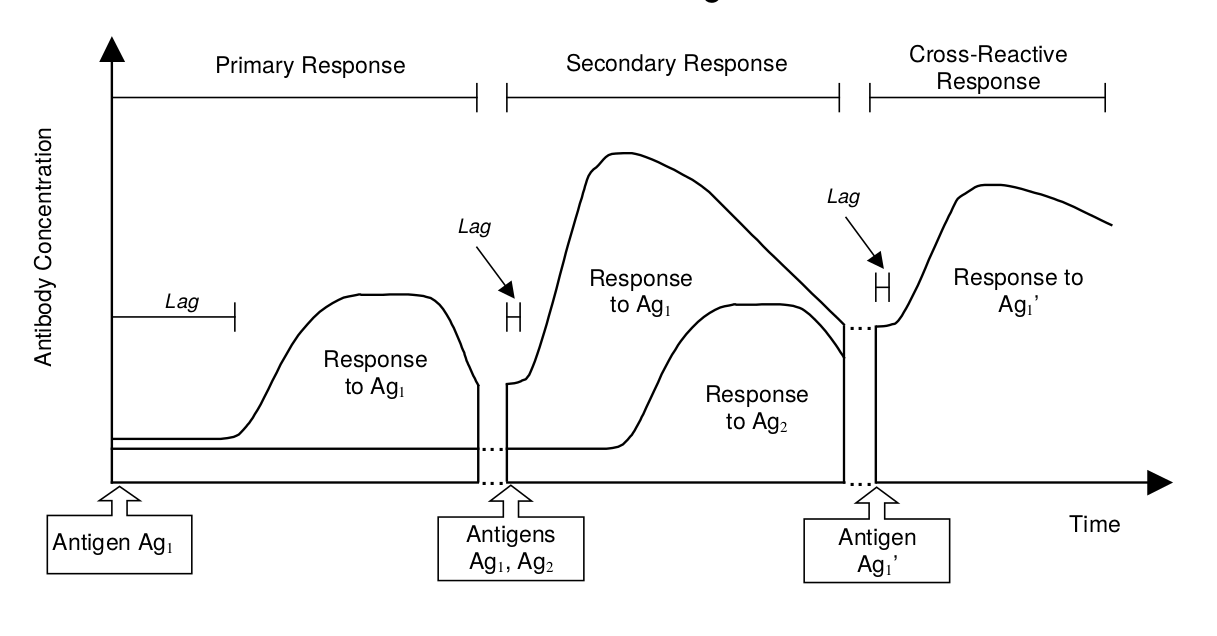
\includegraphics[width=0.95\textwidth]{memory}
        \caption{Respostas primárias e secundárias (De Castro e Timmis, 2002)}
    \end{figure}

\end{frame}

\begin{frame}
    \frametitle{Sistema imunológico adaptativo}
    
    \begin{itemize}
    \item Composto principalmente de células-B e células-T, produzidos na medula
    óssea e no timo, respectivamente.
    \item Células T são subdivididas em: ajudantes, assassinas e supressoras.
    \item Estas células provem três comportamentos que são de interesse computacional:
    Seleção negativa, seleção clonal e hiper-mutação somática.
    \end{itemize}
\end{frame}

\begin{frame}
    \frametitle{Respostas primárias e secundarias}
    
    \begin{figure}[!ht]
        \centering
        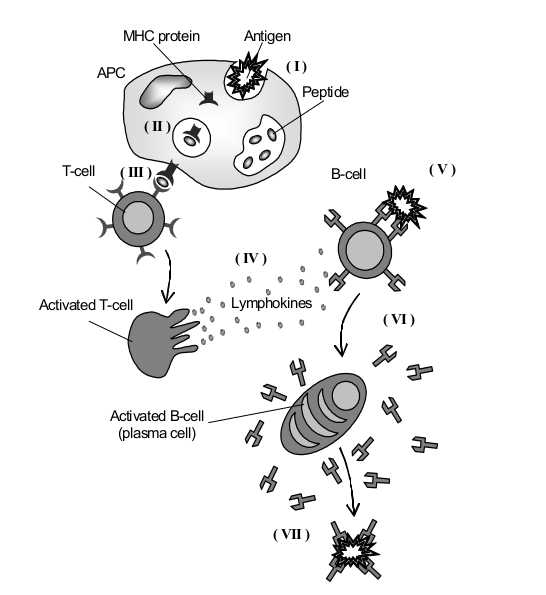
\includegraphics[width=0.45\textwidth]{resposta}
        \caption{Mecanismo de resposta do sistema imunológico adaptativo (De Castro e van Zuben, 1999)}
    \end{figure}
\end{frame}

\begin{frame}
    \frametitle{Seleções}
    
    \begin{description}
        \item[Seleção Negativa:] Processo de seleção que remove células-T que
        reagem ao próprio corpo.
        \item[Seleção clonal:] Modela como a resposta imune ocorre através da
        multiplicação de células-T.
        \item[Hiper-mutação somática:] Mecanismo de mutação para maximizar a
        afinidade.
    \end{description}
\end{frame}


\begin{frame}
    \frametitle{Aplicações}
    
    Sistemas Imunólogicos Artificiais pode ser aplicado nas seguintes áreas:
    \begin{itemize}
        \item Detecção de anomalias e falhas;
        \item Reconhecimento ou Classificação de padrões;
        \item Otimização;
        \item Análise de dados;
        \item Segurança computacional
        \item Aprendizagem de máquina;
    \end{itemize}
    
    Estas aplicações utilizam de algoritmos que serão apresentados a seguir.
\end{frame}

\begin{frame}
    \frametitle{Representação}
    
    Os elementos do sistema imunológico são representados computacionalmente por cadeias de atributos. 
    O tipo de atributo escolhido para representação, pode ser das seguintes formas:
    
    \begin{itemize}
        \item espaço de forma real: cadeia de valores reais
	    \item espaço de forma inteira: cadeia de valores inteiros
	    \item espaço de forma de \textit{Hamming}: composto de cadeia construído com alfabeto finitos de comprimento k;
	    \item espaço de forma simbólica: composto de cadeia onde pelo menos um é simbólico
    \end{itemize}

\end{frame}

\begin{frame}
    \frametitle{Medida de Afinidade}
    
    Para medir a afinidade entre duas cadeias é utilizada o cálculo de distância. Quanto menor a distância, maior a afinidade.
    
    \begin{itemize}
        \item Distância Euclidiana
	    \item Distância de Manhattan
	    \item Distância de Hamming
	    \item r-bits contíguos
    \end{itemize}

\end{frame}


\begin{frame}
    \frametitle{Algoritmos Imuno-Inspirados}
    
    \begin{itemize}
        \item Algoritmos de Geração de Receptores;
        \item Algoritmo de Seleção Negativa;
        \item Algoritmos de Seleção Clonal;
        \item Rede imunológica;
        \item Teoria do perigo;
    \end{itemize}
\end{frame}

\begin{frame}
    \frametitle{Algoritmos de geração de receptores}
    
    Os algoritmos de geração de receptores realizam funções análogas a medula óssea, a qual é responsável pela geração da população de células imunológicas. Estes algoritmos podem ser mais simples ou mais complexos.
\end{frame}
   

\begin{frame}
    \frametitle{Algoritmos de geração de receptores}
    
    \begin{itemize}
        \item Simples: gera uma cadeia de atributos com comprimento L, utilizando um gerador aleatório.
        \item Complexo: gera cadeias de bits a partir de uma concatenação de diferentes componentes genéticos, os quais são selecionados de forma aleatória, cada um de uma biblioteca de genes diferente. \cite{decastro2002}
    \end{itemize}
    
    O comprimento L da cadeia, o número de bibliotecas e os tipos de atributos são todos elementos dependentes do domínio do problema.
\end{frame}

%\begin{frame}
%    \frametitle{Algoritmo de geração de receptores - Complexo}
%    
%    \begin{figure}[!ht]
%        \centering
%        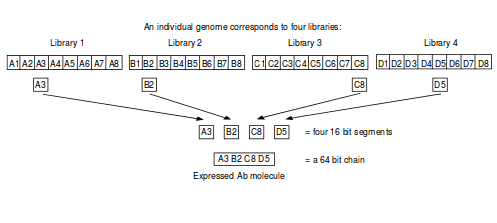
\includegraphics[width=1\textwidth]{GeracaoReceptores}
%        \caption{Algoritmo de geração de receptores utilizando bibliotecas (Perelson et al., 1996)}
%    \end{figure}
%\end{frame}


\begin{frame}
    \frametitle{Algoritmos de Seleção Negativa - NSA}
    
    \begin{itemize}
        \item Aplicado em reconhecimento de anomalias;
        \item Baseado no mecanismo de seleção de células T;
        \item Possui duas etapas: a geração e a detecção.
        \item Componente principal do algoritmo é a regra de detecção. 
    \end{itemize}
\end{frame}

\begin{frame}
    \frametitle{Algoritmos de Seleção Negativa - NSA}
    
    Etapa da geração \cite{decastro2002}
    
    \begin{enumerate}
        \item Definição células próprias como um conjunto de cadeias S; 
        \item Geração de cadeias de forma aleatória; 
        \item Testes a similaridade entre as cadeias pertecentes a S;
        \item Caso a similaridade seja alta então, reconhece uma própria como anomalia, esta cadeia deve ser eliminada.
        \item Caso contrário, a cadeia é selecionada como uma imunocompetente.
    \end{enumerate}
    Similaridade é determinada como alta se for superior a uma limiar.
\end{frame}

\begin{frame}
    \frametitle{Algoritmos de Seleção Negativa - NSA}
    
    Etapa da detecção \cite{decastro2002}
    
    \begin{itemize}
        \item Monitoração do conjunto de cadeia que deseja proteger, para isso utilizar o conjunto de detectores gerados na etapa anterior;
        \item Caso a similaridade seja alta entre o detector e a cadeia. Significa que ocorreu uma anomalia. 
    \end{itemize}
    Similaridade é avaliada com a pré-determinada na etapa de geração.
\end{frame}

\begin{frame}
    \frametitle{Algoritmos de Seleção Clonal}
    
    \begin{itemize}
        \item Aplicado em reconhecimento de padrões, aprendizado de máquina e otimização;
        \item Reconhece uma população de antígenos;
        \item Busca pela otimização de uma ou várias funções, é inspirado na maturação do sistema imunológico;
    \end{itemize}
\end{frame}

\begin{frame}
    \frametitle{Algoritmos de Seleção Clonal - CLONALG}
    
    São três etapas no processo de melhora das soluções utilizando CLONALG:
    
    \begin{enumerate}
        \item Clonagem das soluções;
        \item Hipermutação das novas células geradas;
        \item Seleção das quais possuem maior afinidade em relação ao antígeno. 
    \end{enumerate}
\end{frame}

\begin{frame}
    \frametitle{Algoritmos de Seleção Clonal - CLONALG}
    
    Algoritmo básico\cite{decastro2002}:
    
    \begin{enumerate}
        \item Geração aleatória de uma população inicial de anticorpos;
        \item Dado um conjunto de antígenos, selecione um antígeno $a_{i}$;
        \item Para cada célula $b_{i}$ da população de anticorpos calcule a afinidade entre $a_{i}$ e $b_{i}$;
        \item Criação de uma nova população com os clones dos anticorpos de afinidade mais alta. O número de clones varia de acordo com à afinidade;
        
    \end{enumerate}
\end{frame}

\begin{frame}
    \frametitle{Algoritmos de Seleção Clonal - CLONALG}
    
    Continuação do Algoritmo básico:
    
    \begin{enumerate}
        \item Realização de uma mutação na nova população de clones com uma taxa inversamente proporcional á sua afinidade.
        \item Adiciona estes na população de anticorpos, e seleciona o melhor que irá servirpa como memória do antígeno.
        \item Substituição das células com menor afinidade por novas células geradas aleatóriamente.
        \item Repetir passo 2 em diante até critério de parada seja atingido.
        
    \end{enumerate}
\end{frame}

\begin{frame}
    \frametitle{Exemplos}
    
    Otimizar $min \: f(x)$, onde
    \begin{equation}
        f(x) = \sum_{i=1}^n cos(x^3 - 4x^2 - 2x + 6)
    \end{equation}
    
    \begin{figure}[!ht]
        \centering
        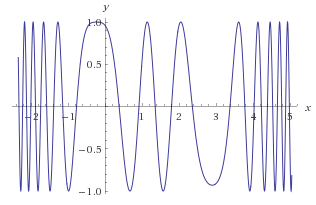
\includegraphics[width=0.45\textwidth]{f1}
    \end{figure}
\end{frame}

\begin{frame}
    \frametitle{Exemplos}
    
    Exemplos retirados de \textit{Clever Algorithms}, por \textit{Jason Brownlee};
    
    \begin{itemize}
        \item  Clonal Selection Algorithm(CLONALG)
        \item Optimization Artificial Immune Network (opt-aiNet);
    \end{itemize}
    
\end{frame}



\section{Refer\^encias}

\begin{frame}[allowframebreaks]
        \frametitle{Referencias}
        \bibliographystyle{elsarticle-num}
        \bibliography{sample}
\end{frame}

\end{document}
